
\documentclass[nooutcomes]{ximera}
%\documentclass[space,handout,nooutcomes]{ximera}

% For preamble materials

\usepackage{pgf,tikz}
\usepackage{mathrsfs}
\usetikzlibrary{arrows}
\usepackage{framed}
\usepackage{amsmath}
%\pgfplotsset{compat=1.16}

\graphicspath{
  {./}
  {algorithms/}
  {../algorithms/}
}

\pdfOnly{\renewenvironment{image}[1][]{\begin{center}}{\end{center}}}

%%% This set of code is all of our user defined commands
\newcommand{\bysame}{\mbox{\rule{3em}{.4pt}}\,}
\newcommand{\N}{\mathbb N}
\newcommand{\C}{\mathbb C}
\newcommand{\W}{\mathbb W}
\newcommand{\Z}{\mathbb Z}
\newcommand{\Q}{\mathbb Q}
\newcommand{\R}{\mathbb R}
\newcommand{\A}{\mathbb A}
\newcommand{\D}{\mathcal D}
\newcommand{\F}{\mathcal F}
\newcommand{\ph}{\varphi}
\newcommand{\ep}{\varepsilon}
\newcommand{\aph}{\alpha}
\newcommand{\QM}{\begin{center}{\huge\textbf{?}}\end{center}}

\renewcommand{\le}{\leqslant}
\renewcommand{\ge}{\geqslant}
\renewcommand{\a}{\wedge}
\renewcommand{\v}{\vee}
\renewcommand{\l}{\ell}
\newcommand{\mat}{\mathsf}
\renewcommand{\vec}{\mathbf}
\renewcommand{\subset}{\subseteq}
\renewcommand{\supset}{\supseteq}
\renewcommand{\emptyset}{\varnothing}
\newcommand{\xto}{\xrightarrow}
\renewcommand{\qedsymbol}{$\blacksquare$}
\newcommand{\bibname}{References and Further Reading}
\renewcommand{\bar}{\protect\overline}
\renewcommand{\hat}{\protect\widehat}
\renewcommand{\tilde}{\widetilde}
\newcommand{\tri}{\triangle}
\newcommand{\minipad}{\vspace{1ex}}
\newcommand{\leftexp}[2]{{\vphantom{#2}}^{#1}{#2}}

%% More user defined commands
\renewcommand{\epsilon}{\varepsilon}
\renewcommand{\theta}{\vartheta} %% only for kmath
\renewcommand{\l}{\ell}
\renewcommand{\d}{\, d}
\newcommand{\ddx}{\frac{d}{dx}}
\newcommand{\dydx}{\frac{dy}{dx}}


\usepackage{bigstrut}


\newenvironment{sectionOutcomes}{}{}

\usepackage{array}
%\setlength{\extrarowheight}{-.2cm}   % Commented out by Findell to fix table headings.  Was this for typesetting division?  
\newdimen\digitwidth
\settowidth\digitwidth{9}
\def~{\hspace{\digitwidth}}
\def\divrule#1#2{
\noalign{\moveright#1\digitwidth
\vbox{\hrule width#2\digitwidth}}}


\title{Functions and Sequences}
\author{Bart Snapp and Brad Findell and Jenny Sheldon}
\begin{document}
\begin{abstract}
Problems about functions and sequences.
\end{abstract}
\maketitle


%\begin{problem}
%Problem
%\begin{freeResponse}
%\begin{hint}
%Hint
%\end{hint}
%\end{freeResponse}
%\end{problem} 

%
%Function given by graph
%Function given by recursive formula
%Function given by table
%Function given by complicated formula
%
\begin{problem}
A \textbf{sequence} is a function with a domain that is a subset of the $\answer[format=string]{integers}$.  

An \textbf{arithmetic sequence} has a constant $\answer[format=string]{difference}$ between consecutive terms. 

An \textbf{arithmetic sequence} is a(n) $\answer[format=string]{linear}$ function. 

An \textbf{geometric sequence} has a constant $\answer[format=string]{ratio}$ between consecutive terms. 

A \textbf{geometric sequence} is a(n) $\answer[format=string]{exponential}$ function. 
\end{problem}



\begin{problem}
Consider a sequence that begins $9, 12$.    
\begin{enumerate}
\item Continue the sequence so that it is an \textbf{arithmetic sequence}:
\[
9, 12, \answer{15}, \answer{18}, \answer{21}, \answer{24}, \dots
\]
\item Assuming that $f(1)=9$, write a recursive formula for the sequence:
\[
f(n+1)=\answer{f(n)+3}\textrm{, for }n\ge\answer{1}.
\]
\item Assuming that $f(1)=9$, write an explicit formula for the sequence: 
\[
f(n)=\answer{3n+6}\textrm{, for }n\ge\answer{1}
\]
\end{enumerate}
\end{problem}


\begin{problem}
Consider a sequence that begins $9, 12$.    
\begin{enumerate}
\item Continue the sequence so that it is an \textbf{geometric sequence}:
\[
9, 12, \answer{16}, \answer{9(4/3)^3}, \answer{9(4/3)^4}, \answer{9(4/3)^5}, \dots
\]
\item Assuming that $f(1)=9$, write a recursive formula for the sequence:
\[
f(n+1)=\answer{f(n)(4/3)}\textrm{, for }n\ge\answer{1}.
\]
\item Assuming that $f(1)=9$, write an explicit formula for the sequence: 
\[
f(n)=\answer{9(4/3)^{n-1}}\textrm{, for }n\ge\answer{1}
\]
\end{enumerate}
\end{problem}



\begin{problem}
The \textbf{$3n+1$ problem} involves integer sequences defined as follows:  Start with any positive integer. Then, if the current term is even, the next term is one half of the current term. If the current term is odd, the next term is $3$ times the current term plus $1$. 

Suppose the first term is 3.  Find the next several terms.  

\[
3, \answer{10}, \answer{5}, \answer{16}, \answer{8}, \answer{4}, \answer{2}, \answer{1}, \answer{4}, \answer{2}, \answer{1}.  
\]

Note that once the sequence reaches $1$, it cycles back to 1 repeatedly.  
\begin{problem}
If we use function notation to describe the sequence, then the recursive rule may be stated as follows: 

\begin{itemize}
\item If $f(k)$ is even, then $f(k+1) = \answer{f(k)/2}$. 
\item If $f(k)$ is odd, then $f(k+1) = \answer{3f(k) + 1}$.  
\end{itemize}

And given $f(1)=3$, it follows that $f(2)=\answer{10}$, $f(3)=\answer{5}$, and so on.  

\begin{problem}
Is there an explicit formula for this function, $f$?  
\begin{multipleChoice}
\choice{Yes, it is linear.}
\choice{Yes, it is quadratic.}
\choice{Yes, it is exponential.}
\choice{Yes, it is trigonometric.}
\choice[correct]{Probably not.}
\end{multipleChoice}

\begin{feedback}
\begin{quote}
\textbf{Claim:} No matter the initial (positive integer) value, the sequence will always reach 1.  
\end{quote}
This claim is often called the \textbf{Collatz Conjecture}, in honor of Lothar Collatz, who introduced the idea in 1937.  As of 2020, the conjecture has been checked by computer for all starting values up to $2^{68} \approx 2.95\times 10^{20}$. The statement is still a conjecture (rather than a theorem) because no one has been able to prove that it holds for \textbf{all} possible initial values.  For more information, see \link[Wikipedia]{https://en.wikipedia.org/wiki/Collatz_conjecture}. 
\end{feedback}

\end{problem}

\end{problem}

\end{problem}



%A Actual (read from the graph or table or computed from a formula)
%E Estimate (estimated from the graph or table or formula)
%Interpolate vs. extrapolate 
%
%M Model
%
%NA not available (we don't have actual data, and our data is insufficient for a good estimate), 
%DNE does not exist 
%


\begin{problem}
The following table shows historical data collected by the National Weather Service.  
\begin{image}
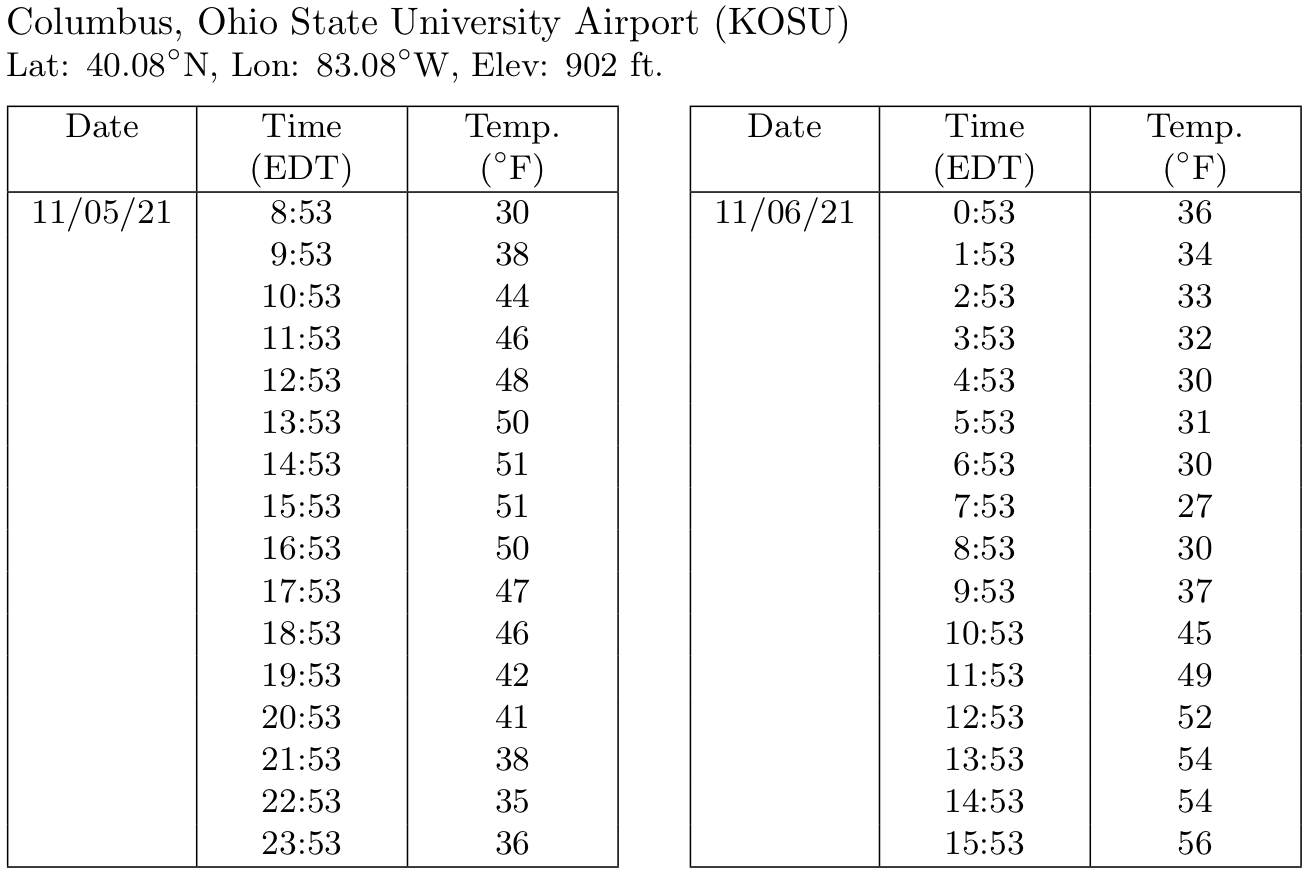
\includegraphics[scale=0.5]{columbusTemp1106.png}
\end{image}
Let $F(t)$ denote the actual or predicted temperature (in degrees Fahrenheit) $t$ hours after the start (at midnight) of November 6, 2021.  

\begin{enumerate}
\item Note that the hourly readings all occur at $53$ minutes after the hour.  For ease of entry, we are going to take 53 minutes as 0.9 hours (though, in fact, 0.9 hours is exactly $\answer{54}$ minutes).  This minor simplification, allows us to write, for example, 
\[
F(0.9) = \answer{36}\text{ and }F(12.9)=\answer{52}.  
\]
\item Negative values of time occur on November $\answer{5}$ or earlier, counting hours backwards from midnight.  For example, 
\[
F(-1.1) = \answer{35}\text{ and }F(-7.1)=\answer{50}.  
\]
\item From real-world data, it is often reasonable to estimate values that are not directly available.  In particular, to \textbf{interpolate} is to estimate between available data values, and to \textbf{extrapolate} is to estimate beyond available values. From this data, for example, we can estimate the following:  
\[
F(9.2)=\answer{32}, F(9.6)=\answer{35}, F(-4.6)=\answer{44}, F(14.5)=\answer{54}\text{, and }F(17)=\answer[tolerance=1]{56}.  
\]
\end{enumerate}

\begin{problem}
From this table, is it reasonable to estimate $F(30)$? 
\begin{multipleChoice}
\choice{Yes, use the formula.}
\choice{Yes, just continue the trend.}
\choice[correct]{Probably not.}
\end{multipleChoice}
\begin{feedback}[correct]
With this small data set, it is not reasonable to extrapolate more than a few hours beyond the available data.  Meteorologists (weather forecasters) use enormous data sets about nearby and historical weather to develop sophisticated models that are usually pretty accurate a few days into the future and somewhat accurate up to ten days.
\end{feedback}

\begin{problem}
Is there an explicit formula for this function, $F$?  
\begin{multipleChoice}
\choice{Yes, it is linear.}
\choice{Yes, it is quadratic.}
\choice{Yes, it is exponential.}
\choice{Yes, it is trigonometric.}
\choice[correct]{Probably not.}
\end{multipleChoice}
\end{problem}

\end{problem}
\end{problem}



%
%Based upon much more sophisticated modeling, the following table shows a temperature forecast for the same location.  
%\begin{image}
%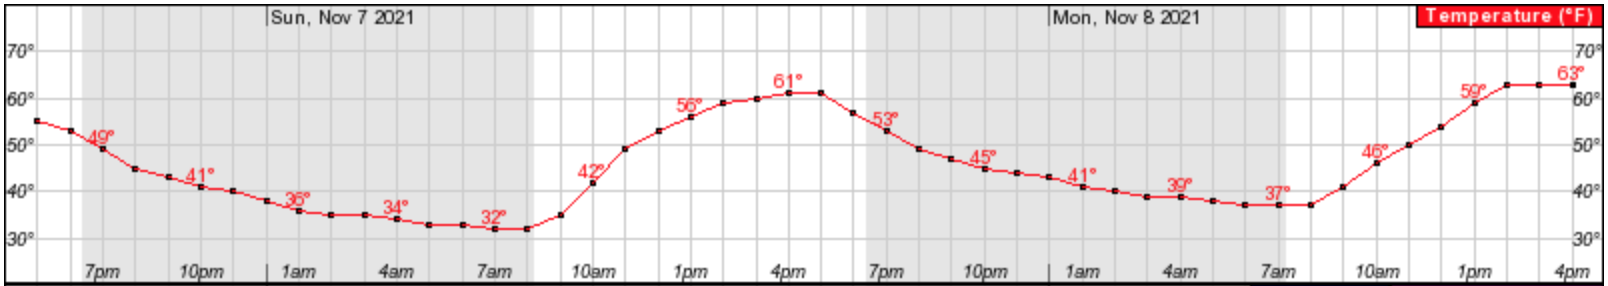
\includegraphics[scale=0.5]{columbusTemp1106F.png}
%\end{image}
%

\end{document}



